\section{Design Implication: A Viewpoint Exposure Report}
\label{sec:design}

The cocoon checks that platforms offer summarise a feed by content categories, which \cref{prop:topic} shows cannot reveal a viewpoint skew. Earlier tools that showed readers the balance of their news diet nudged behaviour a little~\citep{munson2013balance} and raised awareness of filtering~\citep{nagulendra2014visualization}. \Cref{fig:mockup} condenses our results into a design for a \emph{viewpoint exposure report}, shown for the simulated fan of \cref{sec:sim}. Each of its four parts answers to one finding.

\paragraph{Keep interest apart from skew.} The report opens with the topic share and says in words that a large share is interest. The users most at risk of a viewpoint cocoon are heavy viewers of a topic (\cref{sec:sim}); a report that scolds them for the topic would be wrong about the problem and would invite the one remedy that destroys what they value.

\begin{figure}[!t]
  \centering
  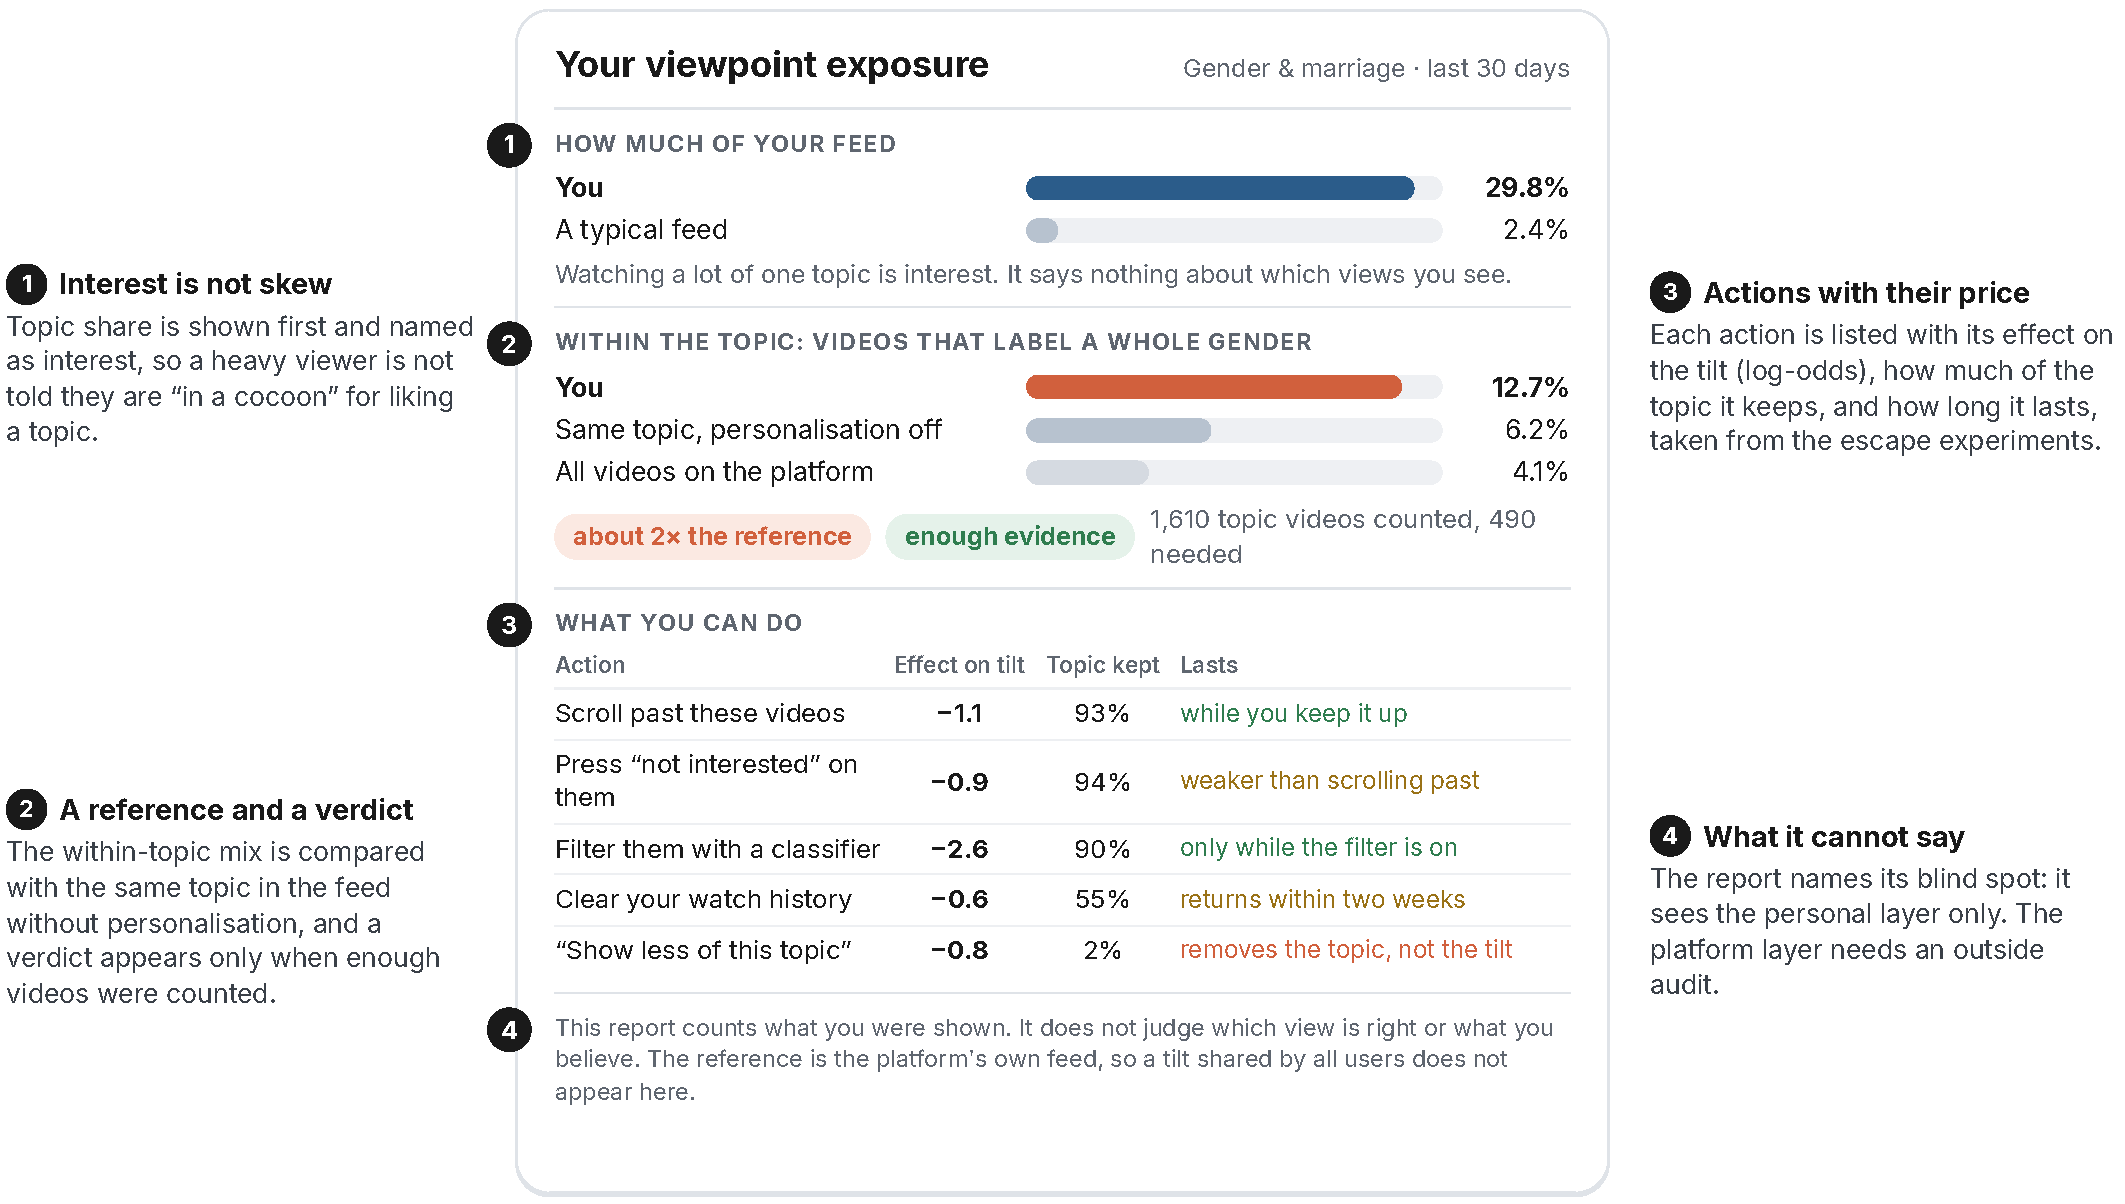
\includegraphics[width=\textwidth]{figures/fig_mockup.pdf}
  \caption{Design of a viewpoint exposure report for one topic, filled with the values of the simulated topic fan (\cref{sec:sim,sec:escape}). The notes at the sides state the finding behind each part. The design has not been tested with users.}
  \label{fig:mockup}
\end{figure}

\paragraph{Compare with a reference, and say when the evidence is thin.} The within-topic share is set beside the same topic without personalisation and beside supply, and a verdict appears only once \cref{eq:detect} is satisfied. The fan of the example has counted 1{,}610 topic videos in a month and passes; a casual viewer would be told ``not enough evidence yet'' for years. Since the reference is the bottleneck (\cref{sec:detection}), it should be computed once by the platform and shown to everyone.

\paragraph{List actions with their price.} Each action carries its effect, the share of topic kept and its persistence, so that the cheap option that removes the topic is not mistaken for a cure. Two changes on the platform's side would make the list shorter and better: reading ``not interested'' as rejection, which turns the weakest explicit tool into the strongest (\str{3} against \str{2}), and offering deletion from history by narrative, not only by video.

\paragraph{State the blind spot.} A report built on the non-personalised reference sees the personal layer only. It says so, and it refrains from judging which view is right or inferring what the user believes.

A platform can produce such a report directly, because it knows each user's exposure probabilities and needs no sampling. A third party would need a classifier, the user's consent to read their feed, and a shared reference. Whether users would read the report as intended, and whether seeing it changes what they watch, are open questions that only a user study can settle.
